\documentclass[11pt,a4paper]{article}
\usepackage[margin=2.2cm]{geometry}
\usepackage{booktabs}
\usepackage{graphicx}
\usepackage{float}
\usepackage[T5]{fontenc}
\usepackage[utf8]{inputenc}
\usepackage[vietnamese]{babel}
\title{Phân tích thực nghiệm bốn cấu hình RC2}
\author{Do Quang Vinh}
\date{\today}
\begin{document}
\maketitle

\section{Thiết lập thực nghiệm}
So sánh bốn cấu hình RC2 trên 72 instance và ba objective: \texttt{finsteps123}, \texttt{infsteps180} và \texttt{cont}.

\begin{table}[H]
\centering
\caption{Các cấu hình được so sánh}
\begin{tabular}{lcc}
\toprule
Cấu hình & B: bound propagation & R: selective refinement \\
\midrule
RC2-Base & Tắt & Tắt \\
RC2+B & Bật & Tắt \\
RC2+R & Tắt & Bật \\
RC2+B+R & Bật & Bật \\
\bottomrule
\end{tabular}
\end{table}

\section{Bảng thống kê}
Mean solve time chỉ tính trên các instance có trạng thái \texttt{ok}; mean total time bao gồm mọi dòng ghi nhận.

\begin{table}[H]
\centering
\scriptsize
\begin{tabular}{llrrrrrrrr}
\toprule
Config. & Objective & N & OK & Fail & Success (\%) & Mean (ms) & Median (ms) & Total (s) & Opt. \\
\midrule
RC2-Base & finsteps123 & 72 & 72 & 0 & 100.0 & 43.89 & 15.78 & 0.04 & 72 \\
RC2-Base & infsteps180 & 72 & 68 & 4 & 94.4 & 1601.03 & 14.96 & 8.19 & 68 \\
RC2-Base & cont & 72 & 57 & 15 & 79.2 & 3489.44 & 13.38 & 27.81 & 57 \\
RC2+B & finsteps123 & 72 & 72 & 0 & 100.0 & 43.63 & 16.48 & 0.04 & 72 \\
RC2+B & infsteps180 & 72 & 68 & 4 & 94.4 & 2126.82 & 31.29 & 8.68 & 68 \\
RC2+B & cont & 72 & 56 & 16 & 77.8 & 4207.11 & 47.41 & 30.00 & 56 \\
RC2+R & finsteps123 & 72 & 61 & 11 & 84.7 & 20.04 & 12.61 & 0.10 & 61 \\
RC2+R & infsteps180 & 72 & 59 & 13 & 81.9 & 40.63 & 12.15 & 7.15 & 59 \\
RC2+R & cont & 72 & 53 & 19 & 73.6 & 3921.01 & 13.29 & 33.11 & 53 \\
RC2+B+R & finsteps123 & 72 & 61 & 11 & 84.7 & 74.97 & 43.89 & 0.25 & 61 \\
RC2+B+R & infsteps180 & 72 & 61 & 11 & 84.7 & 114.27 & 50.05 & 8.17 & 61 \\
RC2+B+R & cont & 72 & 50 & 22 & 69.4 & 3474.43 & 56.57 & 29.55 & 50 \\
\bottomrule
\end{tabular}
\end{table}

\section{Biểu đồ}
\begin{figure}[H]
\centering
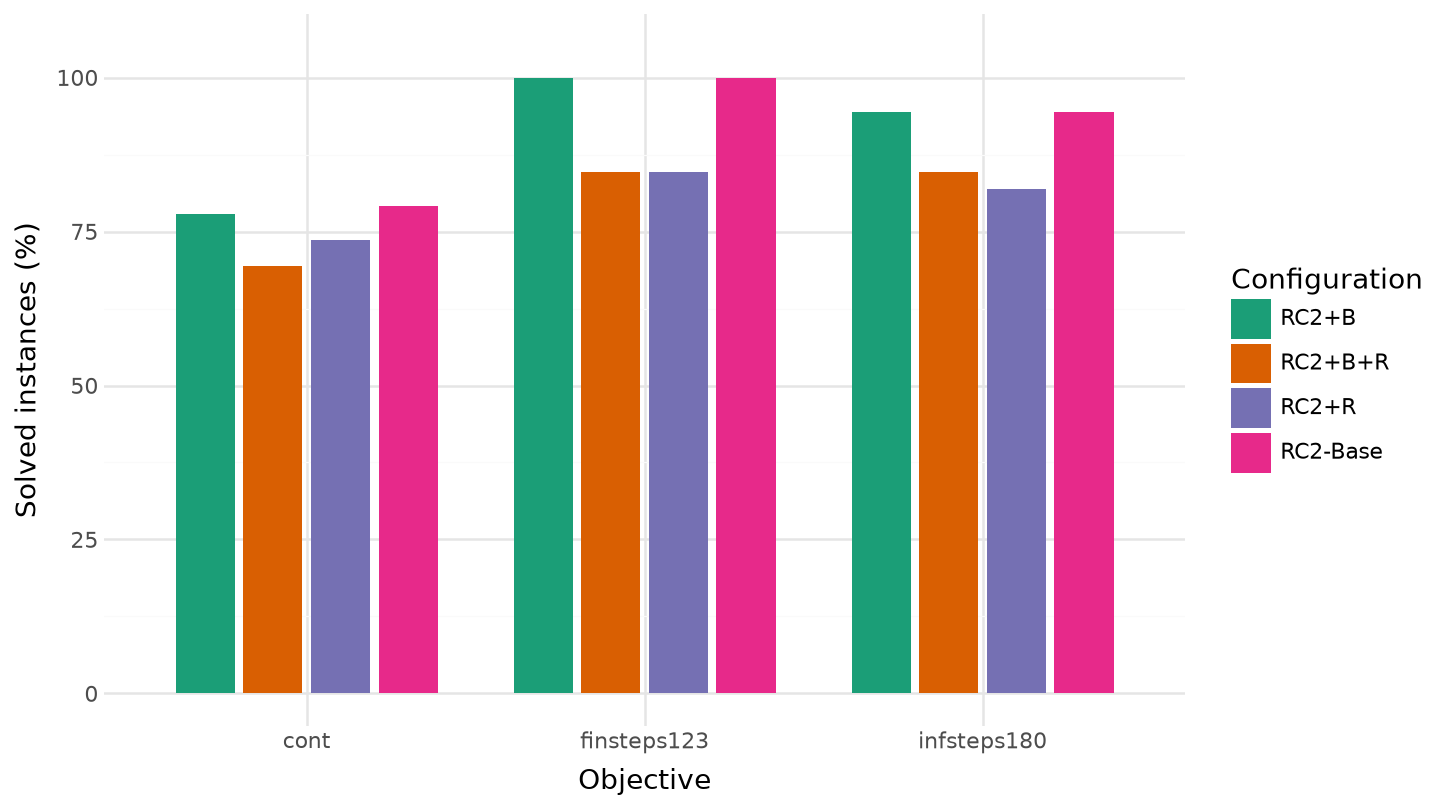
\includegraphics[width=0.9\textwidth]{success_rate.png}
\caption{Tỷ lệ instance giải thành công.}
\end{figure}
\begin{figure}[H]
\centering
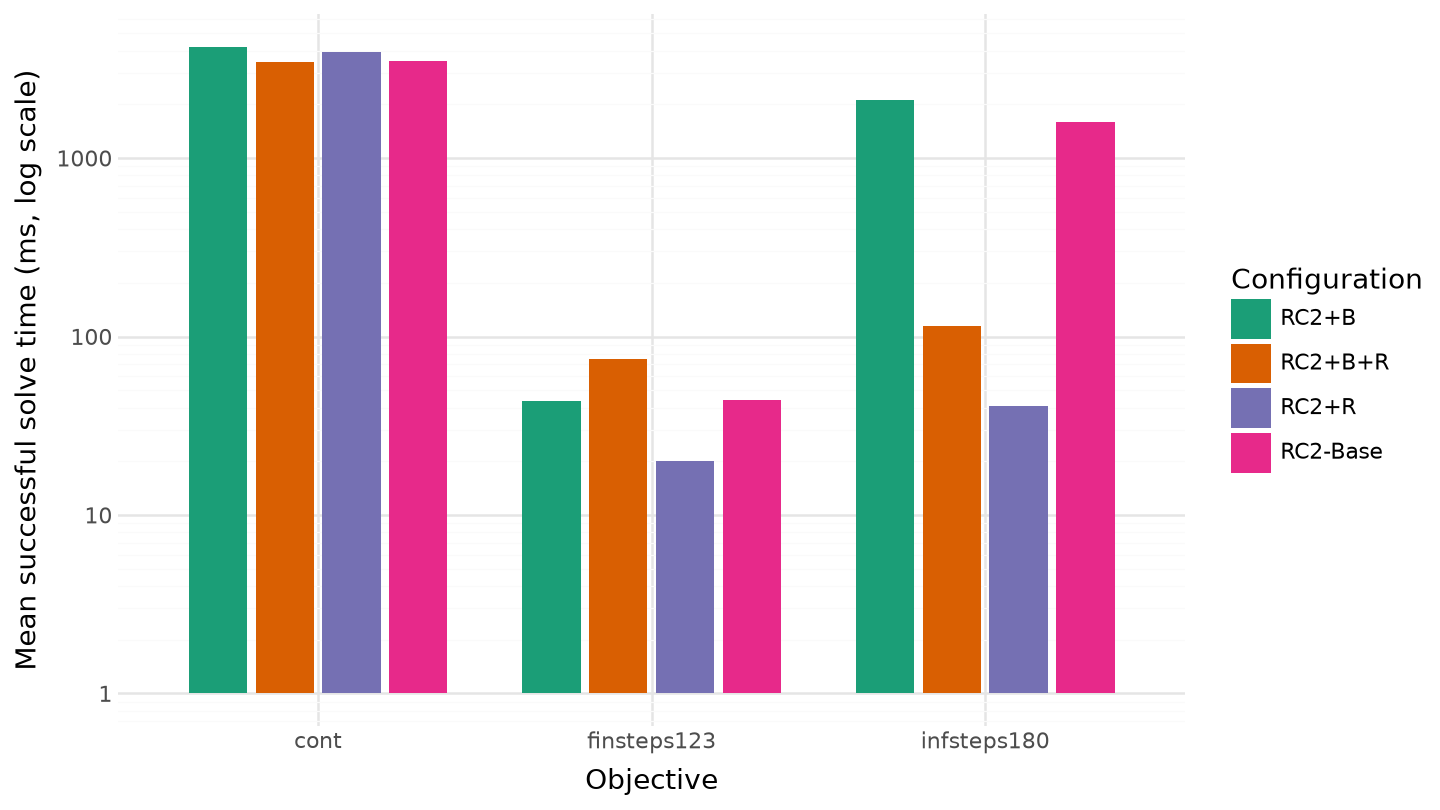
\includegraphics[width=0.9\textwidth]{mean_solve_time.png}
\caption{Thời gian giải trung bình trên các instance thành công.}
\end{figure}
\begin{figure}[H]
\centering
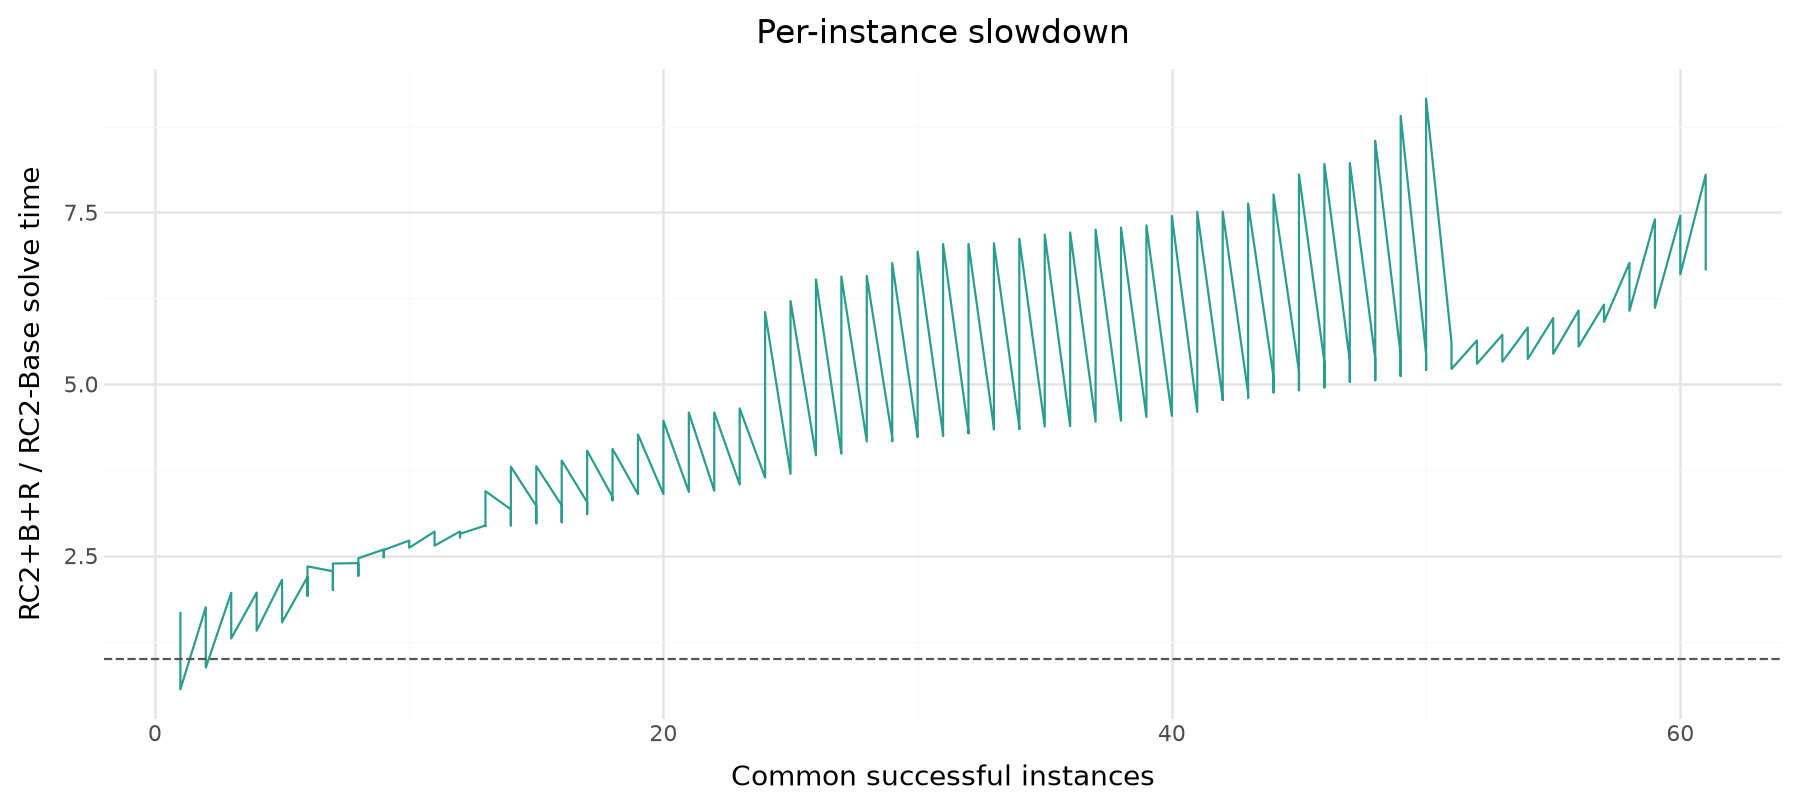
\includegraphics[width=0.95\textwidth]{per_instance_speedup.png}
\caption{Tỷ số thời gian RC2-Base trên RC2+B+R; giá trị lớn hơn 1 nghĩa là RC2+B+R nhanh hơn.}
\end{figure}

\section{Nhận xét}
Với objective \texttt{finsteps123}, RC2-Base có tỷ lệ thành công cao nhất (100.0\%), trong khi RC2+R có median thời gian thấp nhất (12.61 ms).
Với objective \texttt{infsteps180}, RC2-Base có tỷ lệ thành công cao nhất (94.4\%), trong khi RC2+R có median thời gian thấp nhất (12.15 ms).
Với objective \texttt{cont}, RC2-Base có tỷ lệ thành công cao nhất (79.2\%), trong khi RC2+R có median thời gian thấp nhất (13.29 ms).
Các giá trị cost trung bình chỉ được tính trên tập instance giải thành công của từng cấu hình; vì vậy cần dùng tập instance chung nếu muốn kết luận về chất lượng nghiệm. Kết quả hiện tại cho thấy refinement có chọn lọc có thể giảm median thời gian, nhưng việc kết hợp bound propagation không tự động cải thiện tỷ lệ thành công.
\section{Nguồn dữ liệu}
\texttt{RC2-Base}: \texttt{2026-09-27\_19-19-19-RC2-Base}\\
\texttt{RC2+B}: \texttt{2026-09-26\_22-33-15-RC2+B}\\
\texttt{RC2+R}: \texttt{2026-09-27\_18-25-54-RC2+R}\\
\texttt{RC2+B+R}: \texttt{2026-09-27\_23-45-00-RC2+B+R}\\
\end{document}
